%!TEX root = paper.tex

\section{BLE Fingerprinting Toolkit}
\label{sec:methodology}

BLE poses a new and significant threat to the location privacy of
mobile device users. Furthermore, the BLE MAC address randomization doesn't hide the hardware
fingerprints of the BLE radio transmitting those packets. An attacker can profile the hardware 
fingerprint of the BLE radio and track the user.

In this section, we develop a systematic toolkit to extract such hardware fingerprints of the BLE 
wireless transceivers in the portable electronic devices like smartphone and smartwatches. First, we explore and understand ways to fingerprint the wireless transceivers. Next, we develop a 
methodology which can be used to extract the hardware imperfection information from the BLE transmissions, wherein, 
we develop a joint estimation technique to extract the identifying information accurately. 

\subsection{BLE has WiFi-like signal imperfections} %{{{
\begin{figure}[t!]
    \centering
    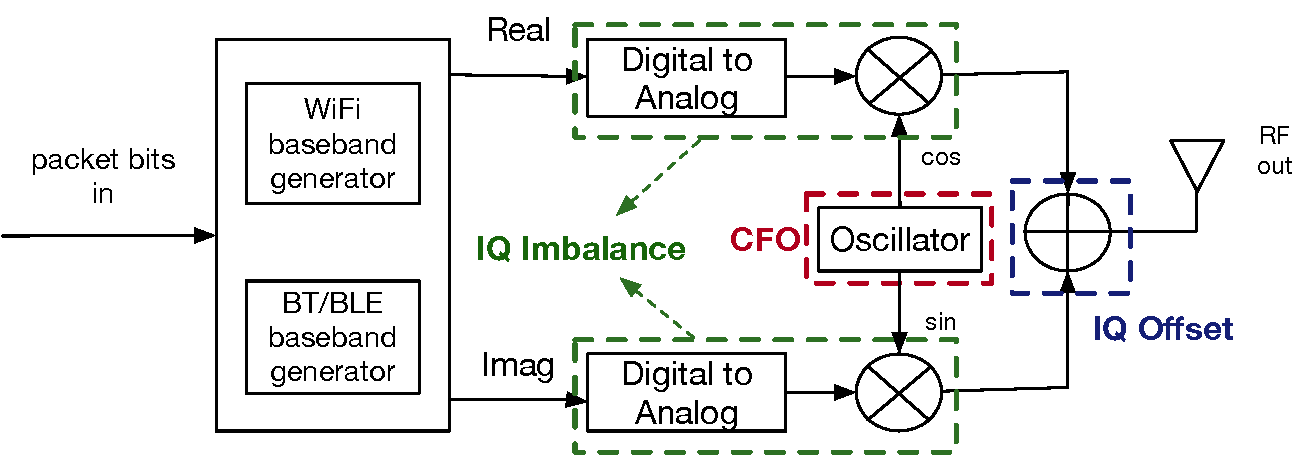
\includegraphics[width = \linewidth]{plots/IQchain.pdf} 
    \caption{Architecture of WiFi/BLE combo chipsets}
    \label{fig:iq_arch}
\end{figure}

\if 0
\todo{move this to related work as well}
Several hardware imperfections have been explored for RF fingerprinting in the literature. 
For instance, transient portion of the signal has been proposed as a unique signature to 
classify different wireless devices~\cite{extraction_rehman, transientID_danev} even Bluetooth
signals~\cite{transientBT_Hall}. However, the transient portion of BLE and Bluetooth signals
is only about 2 microseconds and contains insufficient information to uniquely identify 
a device among tens of devices. Modulation-shape features have also been explored for RF
fingerprinting devices such as RFID transponders~\cite{rfidphysical_danev}. However, 
the Gaussian shape in GFSK modulation of BLE signals is generated digitally in most 
personal electronic devices such as phones, and thus, cannot be used as a unique fingerprint.
\fi
% Now the question is: Do these hadrware imperfections (CFO and IQ imperfection) that have 
% been demonstrated to be the most effective in RF fingerprinting, exist in BLE signals as well?
%Interestingly enough, even though BLE signals are much less complex than WiFi, many mobile devices introduce the  same complex hardware imperfections in BLE as they do in WiFi. This is 
%\todo{talk suitability and other features}


Physical layer fingerprinting is possible due to each radio having unique
hardware imperfections in its transmitter chain. We present the popular WiFi RF-fingerprints
used in the literature, as there has been extensive work on the WiFi fingerprinting. 
% In the WiFi literature, CFO and IQ imperfections (IQ origin offset and IQ imbalance) are 
% two well recongized features which have been shown to be the most separable features for 
% WiFi fingerprinting~\cite{Brik_radiometric}. 
The source of hardware fingerprint for WiFi can be attributed to the complex modulation used by WiFi. 
%
WiFi chipsets have a unique fingerprint because they require generation of
complex multi-carrier modulation waveform. To generate this waveform, many
mobile device chipsets use an \iq modulation architecture shown in
Figure~\ref{fig:iq_arch}.
%
In the WiFi literature, \emph{Carrier Frequency Offset (CFO)} and \emph{IQ imperfections} (which
consists of IQ offset and IQ imbalance) are well recognized features which have been shown to be the most separable features for 
WiFi transmitter fingerprinting~\cite{Brik_radiometric}. 

 \emph{CFO} is the offset in the carrier
frequency generated by the local-oscillator. 
It is caused by imperfections in the radio's
crystal oscillator; specifically, the crystal and the tolerance of oscillators
yields unique CFO even for the devices from the same make and model. 
The carrier frequency is fed to the mixer, which multiplies it with the complex base-band signal and
transmits it, thereby carrying the offset as a feature in the transmission. The \emph{IQ imperfections} result from the following phenomenon: IQ offset
comes from the carrier frequency signal at the mixer leaking into the transmit signal, 
or the baseband signal having a DC offset. % This can add a fixed complex term to the I and Q sample (shift the
%center of constellation).
IQ imbalance occurs because of a mismatch
between parallel analog components of RF chain in I (in-phase) and Q
(quadrature) signal path.% This makes the phase and amplitude of I and Q path
%asymmetric. 


%In this type of
%transmitter, the I (real) and Q (imaginary) parts of the waveform are generated
%by the digital baseband. The real and imaginary parts of the signal are
%eventually mixed with a carrier frequency ($f_c$), where real part is
%multiplied cosine ($cos(2\pi f_c t$) of the carrier frequency and vice versa
%for imaginary part.

\subsubsection*{Mobile devices use combo BLE/WiFi chips}
%
We make an interesting observation, which allows us to leverage existing WiFi fingerprints for BLE,
 i.e. WiFi and BLE share the same transmit chain in the smartphones.
Specifically, in order to save cost of RF hardware, high power devices (e.g. smartphones) are
equipped with combo chips which have both BLE and WiFi digital baseband modem, and
share the common I/Q front-end to transmit and receive the signals 
(Figure~\ref{fig:iq_arch}).
%
Combining the transceiver front-end reduces the device's overall size, power-consumption, and serves as a
point to synchronize both protocols' 2.4~GHz transmissions, so they do not
interfere with each other.
%
However, an unintended result of this hardware design choice, is that BLE
transmissions contain the same imperfections that have been previously exploited to fingerprint WiFi transmitters.
%
However, can we extract the CFO and IQ imperfections from the
BLE signals to uniquely fingerprint the devices?


\subsection{BLE is difficult to fingerprint} %{{{
\label{sec:motivation:diff}

\begin{figure}
    \centering
    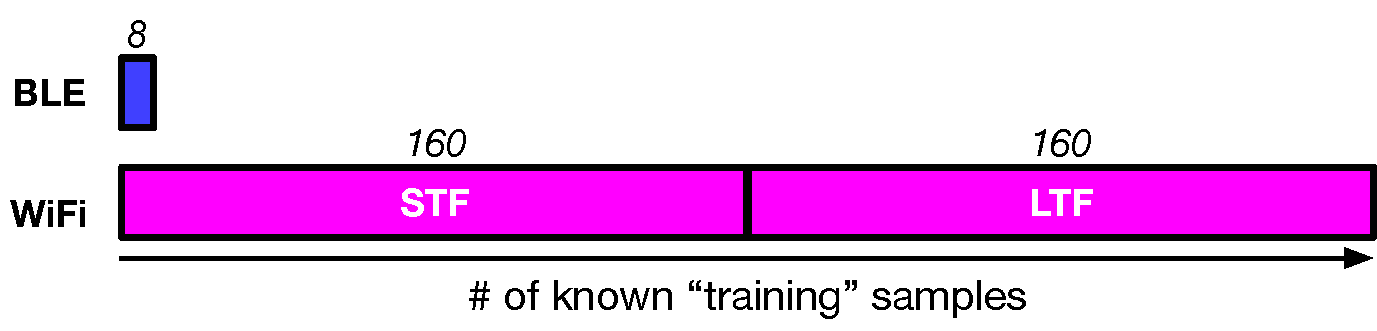
\includegraphics[width=\linewidth]{plots/knownsamples}
    \caption{
      BLE packets have very few known samples for physical layer fingerprinting.
    \label{fig:2}
  }
\end{figure}


%
%The reason is, BLE is an extremely low-energy protocol: BLE's physical-layer
%signal is designed to require simple hardware to transmit and receive messages.
% 



% BLE signals are generated by representing the bits as basic  Gaussian Frequency Shift Keying (GFSK) modulation, where $f_0$ means bit $0$ and $f_1$ means bit $1$. 
% Although symbols in a BLE signal are not modulated in I/Q domain, often the CFO and IQ imperfections are embedded in the BLE signals as a part of the transmitting them from an I/Q modulator based radio. Ideally, an attacker would need to receive these samples, and extract these 
% impariment using the simple FSK signal. The standard BLE receivers can decode the 
% packet without explicity correcting for CFO or IQ imperfections as FSK is a non-IQ modulation scheme. 
% There are two key challenges with extracting CFO and IQ imperfections:
Extracting the CFO, IQ offset and imbalance of the front-end from the BLE signals is often challenging.  
%
Primarily, as the design of BLE's physical layer is so simple that it cannot 
estimate the CFO and IQ imperfections accurately.
The BLE signals are simple narrowband Gaussian Frequency Shift Keying (GFSK) signals which makes it challenging to estimate
CFO and IQ imperfections accurately. For instance, the WiFi signals are wide-band signals
whose decoding algorithms require correcting for CFO and IQ imperfections to achieve accurate decoding. As a result, signal features such as LTF or multiple subcarriers have been exploited to estimate these imperfections accurately. For example, WiFi signal has a bandwidth of 20 MHz, wherein, intuitively the phase change over the 20 MHz wave is used to measure the 
carrier frequency offset, therefore providing a much more accurate measurement compared to 1 MHz bandwidth of BLE. Moreover, BLE transmissions do not require a significant number of known ``training''
samples for a receiver to use to correct for imperfections before decoding. As a result, only a short 8 us preamble is considered in BLE packet design.

%In constrast, BLE signals use FSK modulation, where in the receiver uses the preamble to identify the mid-point of the two frequency used for data modulation, and uses that as a calibration point, to decode bits as 1 or 0. 

%  
These limitations make it difficult to apply existing physical-layer techniques~\cite{vohuuusrp,Brik_radiometric,deviceID_kose,Intrusion_hall,suskitransient,deeplearning_merchant,lora_robyns,gopalakrishnan2019robust}
to fingerprint BLE.
%
The problem is, these techniques have been developed for protocols, such as
WiFi, that have signal features which make it easy to accurately measure and compensate these imperfections.
%
For instance, Figure~\ref{fig:2} shows a comparison of the length of a typical
BLE beacon packet compared to a typical WiFi packet.
%
BLE packets only include 8 known samples, whereas WiFi packets include 
a total of 320 known samples. Consequently, using preamble-based methods to extract CFO from BLE signals yields less accuracy compared to WiFi.


\vspace{0.5em}
\noindent\textbf{Existing coarse CFO estimation in BLE receivers}
Coarse-grained CFO compensation is implemented in BLE receivers.  They
implement this by analyzing the small number (8) of known samples in the
preamble of each packet.
%
BLE receivers estimate CFO from these bits by averaging the frequencies of each
FSK symbol in the preamble. Another popular CFO algorithm used in the Texas
Instruments CC2400 BLE chipset averages the minimum and maximum frequency of
the preamble~\cite{cvtracksun}.
%
Since the preamble is an 8-bit sequence of consecutive 0 and 1, the frequency
of preamble is symmetric.  Therefore, ideally the average of the frequencies in
preamble must be 0. If there exists CFO, this average will be an estimate of
CFO.
%
However, as these techniques only rely on 8 samples in the preamble. Consequently, they do not produce an
accurate estimate of CFO---leading to confusions between device fingerprints.
%
Indeed, with only 8 samples, the theoretical limit of CFO accuracy 2 kHz assuming 3 degree phase noise. Moreover, inaccurate or coarse-grained compensation of CFO, significantly affects I/Q offset and imbalance estimation as it causes a time-dependent phase
shift which distorts the \iq constellation

\subsubsection*{Novelty of our technique}
\noteby{NB-7}{
Our technique is the first-ever physical layer identification method that can estimate I/Q imperfections of BLE signals, in addition to high-precision CFO estimates. 
%
We did so by solving two major challenges.
%
Firstly, since CFO and I/Q imperfections are interrelated, I/Q imperfections cannot be estimated accurately unless we obtain an accurate CFO estimate.
%
To resolve this, we present a novel approach that jointly estimates CFO and I/Q imperfections, ensuring on completion both parameters are precisely estimated.
%
Lastly, accurate estimation of CFO and I/Q imperfections is difficult for BLE signals because the known packet segment (preamble) is very short.
%
We addressed this challenge by re-encoding the received bitstream into a BLE signal with varying CFO and I/Q imperfections, until we find CFO and I/Q estimates such the re-encoded signal matches the original received signal.
%
}



% \subsection{BLE is ubiquitous }

% Our goal is to identify the wireless transceiver, which could leak the location and be able to identify them. Most
% transcevivers today use MAC address randomization to enable to privacy. Hence, we focus on building a methodlogy to
% extract the physical tranceivers fingerprints to identify the emission and thereof their proximity.

% A natural way to perform finger-printing would be to leverage WiFi signals; as there has been extensive literature on extracting the WiFi fingerprinting. However, suprisingly the WiFi transceiver are quiet i.e. they only transmit when the user uses the portable devices, and performs in-frequent beacons. Furthermore, WiFi transceivers are long-range making it hard to find proximity of the user. Finally, some of the portable devices do not have WiFi transceivers. Thus using WiFi wouldn't scale as an attack.

% On the otherhand, bluetooth low energy (BLE) tranceviers are part and parcel of all portable devices. Next, the BLE emissions are short range making them vulunerable in providing the proximity of the user. Finally, the BLE was designed for advertisement i.e. they beacon frequently and futhermore, many devices use BLE for continuity protocol
% \todo{descirbe the protocol}. In summary, BLE emissions are all ubiquitious, pervasive and beaconing frequently. However, the BLE protocol randomizes the MAC address every 15 minute to provide privacy to the user. However, they are still vulnerable to the physical layer fingerprinting. 


% \subsection{Novel Technique to Extract the RF fingerprints using the BLE}

% We present first a new physical layer fingerprinting technique that
% can uniquely identify BLE devices.
% %
% We first describe why surprisingly, even though BLE signals are much less
% complex than WiFi, many mobile devices introduce the same complex hardware
% imperfections in BLE as they do in WiFi.
% %
% Then we present a new algorithm to robustly and accurately extract these
% WiFi-like imperfections from BLE packets.
% %
% The key contribution of our algorithm is overcoming the primary limitation of
% BLE physical layer fingerprinting: its short known samples in its preamble
% (Section~\ref{sec:motivation:diff}).

%}}}

\subsection{Accurate Estimation of CFO \& \iq imperfections in BLE} %{{{
\label{sec:methodology1}
\begin{comment}
We know that combo chips cause WiFi-like imperfections in BLE transmissions.
%
However, estimate

So far, we described although combo chips introduce WiFi-like imperfections in BLE transmissions
from mobile devices, estimating these imperfections in a capture of a BLE transmission is extremely challenging. 
\end{comment}
Existing methods to estimate CFO \& I/Q imperfections in both WiFi and BLE provide low accuracy.
%
Opportunistically to fingerprint a larger number of BLE devices, we need high accuracy estimation of these WiFi-like imperfections.
%
\begin{comment}
are insufficient --- they don't provide the precision necessary for fingerprinting a large number of devices.

extract these imperfections from either WiFi or BLE signals, does not provide the precision required for RF fingerprinting a large number of devices. 

%
Therefore, the real challenge is how to measure these imperfections accurately from a BLE signal. 
\end{comment}
In this section, we present a new algorithm to robustly and accurately extract these WiFi-like imperfections from BLE packets.

%
%These hardware imperfections have been demonstrated to be the most important
%characteristics for building RF fingerprinting systems for WiFi devices.  As a
%result, we can take advantage of these previously explored hardware
%imperfections to build our physical layer attack on BLE devices.
%

%
%There is no existing technique for estimating the mentioned imperfections for
%BLE devices with the granularity and accuracy which is needed for the task of
%device identification.
%
%

%As discussed in Section~\ref{sec:background}, CFO, IQ offset and IQ imbalance
%are important hardware characteristics that can be leveraged to uniquely
%identify this architecture as proposed by prior works for fingerprinting WiFi
%devices as well. However, the challenge is how we can estimate these
%imperfection parameters accurately and fine-grained to fulfill the device
%identification task. WiFi signal eases this job by having specific signal
%features such as LTF and multiple subcarriers (and also WiFi chipsets report
%CSI which can easily be used to estimate these imperfections). This is mainly
%because fine-grained estimation and compensation of CFO and IQ imperfections is
%an unavoidable step in decoding WiFi signal. If CFO compensation is not
%accurate in WiFi decoding, IQ samples will rotate by time, and if IQ
%imperfection is not compensated, the shape of constellation will change. Both
%of these will drastically affect the decoding process since symbols are
%modulated in IQ domain. As a result, the mentioned signal features have been
%anticipated and there is a huge body of work on how to etimate these
%imperfections accurately for WiFi signals (not only for RF fingeprinting, but
%also for other purposes).


%In order to build a robust algorithm, we would start from the physics of the
%BLE architectures and build algorithms to capture hardware impariments to
%uniquely identify each radio. We present a novel algorithm to recover the
%hardware impairments which WiFi based RF fingerprinting relies on.
%Specifically, we would discuss how to extract the accurate hardware
%impairments such as CFO, IQ offset and IQ imbalance with just using the BLE
%transmissions which have narrow bandwidth with short packet sizes and short
%preamble length. 

%Next, we un-cover that not all devices use IQ architecture or popular architecture used by WiFi transceivers. In order to reduce power, the  reveal that BLE-only chipsets do not use the commonly known transmitter architecture and consequently, do not have many of the well-known hardware impairments. As a result, we porpose a new technique for profiling those architectures. Finally, we illustrate the overall flow of our fingerpriting methodology.
\begin{comment}
and we show that the second technique can be used to fingerprint any kind of Bluetooth transmitter, regardless of the transmitter architecture.
\end{comment}

%Hardware Impairment estimation for WiFi/BLE Combo-chips}

% Talk about the combo chip first and explain how smartphone use those and therefore we can use the similar hardware impariments as IQ chipsets.

% this sentence says everything in one sentence slow it down, talk about WiFi devices first, show a figure with the architecture of the WiFi chipset to explain

%Practical hardware concerns have made the usage of I/Q path in transmitter architecture including WiFi chipsets, a desirable choice. In this kind of architecture, I and Q data are generated in different paths and eventually they are mixed with the carrier frequency. On the other hand, the hardware imperfections caused by this kind of hardware design, including CFO, IQ offset and IQ imbalance [CITE], have been proposed as important hardware characteristics which can be used to distinguish different devices. Naturally, the devices equiped with both BLE and WiFi technology (e.g. smartphones), utilize the same piece of hardware as a combo chipset for sending both BLE and WiFi packets as shown in Fig. XXXX. The reason lies in cost efficiency, simplifying board design, and optimizing die size and on-board area. As a result, we can take advantage of previously explored hardware imperfections (CFO, IQ offset and IQ imbalance). \\

%In previous works, CFO, IQ offset and IQ imbalance [CITE] have been proposed as important hardware characteristics which can be used to distinguish different devices. 


% Next talk about WiFi decodes the CFO etx and how it does, can we apply similar technique to BLE, we cannot, why?
% talk about how BLE is challenging with narrow bandwidth, short preamble makes it hard to detect CFO, if similar techqnieu as WiFi is applied what is the resolution you would get and would it resolve the devices (make the problem look hard)

%Measuring these harware imperfections is an unavoidable stage in decoding WiFi packets since it can significantly affect the decoding error if the receiver does not compensate them. As a result, measuring these imperfection has been heavily researched for WiFi signals. More than that, pecific arrangements have been devised in WiFi protocol to make the estimation of these imperfections easy and accurate. On the other hand, decoding the simple GFSK modulation which is used in BLE and Bluetooth, is not affected by the aforementioned imperfections severly. Therefore, there has not been any attempt on measuring these impairments accurately for a BLE or Bluetooth signal. Also, using the same techniques for estimating impairments as WiFi, will result in a much lower accuracy of estimation because of having a narrowband (without subcarrier) short signal (typically a few hundreds of microseconds) with a very short premble (8 microseconds). For instance, we employed the technique that is used in Bluetooth test equipments which exploits the preamble to estimate CFO [CITE]. That is, simply we take the average of frequencies in the preamble. Since preamble is an 8-bit sequence of consecutive 0 and 1, the frequency of preamble is symmetric. Therefore, ideally the average of thh frequencies in preamble must be 0. If there exists CFO, this average will be an estimate of CFO. However, this estimation is not precise and robust as it only relies on a an 8-microsecond preamble. The resulting standard deviation of the measured CFO was 1.5 KHz (we averaged the CFO standard deviation across 20 different devices). This standard deviation is huge for performing the task of RF fingeprinting and will end up in low accuracy of identifying devices based on RF fingerprints. We also tried the MINMAX algorithm described in [CITE] but it yields even worse standard deviation.\\

% then propose your solution layer by layer, first layer to increase the resolution your idea is to use entire packet, which requires you to decode the data and then reconstruct the receive singal witout hardware impariment and use that to estimate the impariements. 

%In WiFi it is necessary 
%features such as LTF and multiple subcarriers (and also WiFi chipsets report
%CSI which can easily be used to estimate these imperfections). This is mainly
%because fine-grained estimation and compensation of CFO and IQ imperfections is
%an unavoidable step in decoding WiFi signal. If CFO compensation is not
%accurate in WiFi decoding, IQ samples will rotate by time, and if IQ
%imperfection is not compensated, the shape of constellation will change. Both
%of these will drastically affect the decoding process since symbols are
%modulated in IQ domain.

% Extra text {{{
\if 0
Unlike WiFi, decoding BLE or Bluetooth signals does not require accurately
estimating and compensating for CFO and IQ imperfections.
%
Even several kHz of CFO will not affect the decoding process of BLE's FSK
signals. Also, as FSK symbols are not modulated in IQ domain, IQ imperfections
does not significantly the affect BLE decoding process.
%
As a result, unlike WiFi, there was no need to embed any known signal feature
in BLE signal to provide necessary means for accurate and fine-grained
estimation of these imperfections.
%
For instance, BLE preamble is only 8 bits (8 microseconds) which is much
shorter than WiFi, it uses the simple GFSK modulation, and there does not
exists multiple subcarrier in BLE signal or CSI in BLE chipsets. This
simplicity of BLE signal leaves us in a situation where estimating these
imperfections for BLE signals is much more challenging than WiFi.
The consequence of this fact is that existing techniques for fine-grained
estimation of CFO and IQ imperfection of WiFi signals, either cannot be
adopted or will not result in fine-grained imperfection estimation for BLE
signals.  Moreover, techniques that are specifically designed for CFO
estimation of BLE or Bluetooth signals provides only a very coarse-grained
estimation which is not sufficient for device identification task at all, and
not surprisingly, there has not been any attempt on estimating IQ imperfection
for BLE or Bluetooth signals as it is not needed for decoding.
\fi
%}}}


%

%
% ADS: Sounds fun but no space
%
%We tried simply extending this method to take advantage of the entire packet
%and take average across frequencies of equal number of 0's and 1's. However,
%we did not see any significant benefit for doing that.

\subsubsection{Goals}
%
To implement an accurate BLE CFO fingerprinting algorithm that can also estimate I/Q imperfections, our algorithm must have two key properties.
%
First, instead of relying on the 8 known samples in the preamble, our goal is
to utilize the entire packet ($\sim$370 samples).
% in order to diminish the
%effect of noise and provide more information and granularity for accurate
%imperfection estimation.
These additional samples will provide a theoretical CFO accuracy of 
about 40 Hz compared to the 2 KHz of coarse-grained
estimation.
%
Second, it must jointly estimate CFO and I/Q imperfections to prevent the
mutual effects on each other's estimation.

\subsubsection{Overview}
%
\begin{figure}[t!]
    \centering
    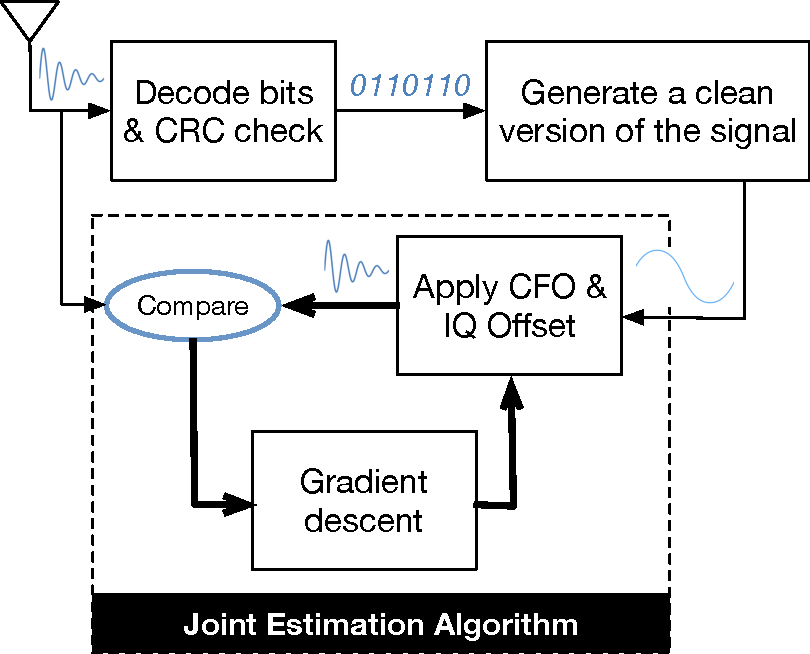
\includegraphics[width = \linewidth]{plots/jointestimation.pdf} 
    \caption{Overview of our hardware imperfection estimation algorithm. The received signal is first decoded. Then the decoded bits are modulated as a perfect BLE signal. Finally, hardware imperfections are added to the perfect signal until the signal matches the actual received signal.}
    \label{fig:jointestimation}
\end{figure}

Keeping these two goals in mind, we develop an algorithm to estimate CFO and IQ
imperfections for BLE signals.
%


To be able to take advantage of the entire packet properly, we first
decode the packet. Our insight is that because GFSK modulation is robust to CFO, IQ imperfections and noise,
we will be likely to decode the packet correctly, and this can be checked with
BLE's CRC.
%
Once we have the decoded data, we can reconstruct an ideal version of
the transmitted signal.
%
Then we jointly insert the hardware imperfection parameters (CFO and I/Q offset and imbalance) in the
mathematical model of the ideal signal. Then we keep modifying those
imperfection parameters until the ideal representation of the signal
looks like the actual captured signal. Brute force search for these hardware imperfection parameters and trying all possible values has a huge computational complexity as the search space for
these imperfection parameters is vast. As a result, we use optimization techniques to efficiently move towards the optimal value of these parameters as shown in Figure~\ref{fig:heatmap}.

%to WiFi. Therefore, decoding can be done properly without compensating hardware
%imperfections.  

%However, to build an algorithm for estimating these fingerprints accurately and robustly, despite the existing techniques, we cannot rely on the preamble since it is very short for BLE and also, there is no notion of subcarrier in BLE technology. For instance, we employed the technique that is used in Bluetooth test equipments which exploits the preamble to estimate CFO~\cite{?}. That is, simply we take the average of frequencies in the preamble. Since preamble is an 8-bit sequence of consecutive 0 and 1, the frequency of preamble is symmetric. Therefore, ideally the average of the frequencies in preamble must be 0. If there exists CFO, this average will be an estimate of CFO. However, this estimation is not precise and robust enough as it only relies on a an 8-microsecond preamble. The resulting standard deviation of the measured CFO was 1.5 KHz (we averaged the CFO standard deviation across 20 different devices). This standard deviation is huge for performing the task of RF fingeprinting and will end up in low accuracy of identifying devices based on RF fingerprints. \\

%Instead of relying on preamble or specific short parts of the packet, we can benefit from the entire packet to make a robust and accurate imperfection estimator since using the entire packet helps in diminishing the effect of noise as well as providing more information and granularity to estimate imperfections accurately. Although for being able to take advantage of the entire packet properly, we need to first decode the packet. Note that thanks to simple GFSK modulation, hardware imperfection does not cause decoding error as opposed to WiFi. Therefore, decoding can be done properly without compensating hardware imperfections. Once we have the decoded data, we can reconstruct the ideal signal. The high level idea is that we insert hardware imperfection parameters in the mathematical model of the ideal signal. Then we keep changing those imperfection parameters until the mathematical representation of the signal looks like the actual captured signal. However, since the search space for these imperfection parameters is vast, we use optimization techniques to move towards the optimal value of parameters efficiently. \\
%Although we consider GFSK modulation in this paper, the idea behind this method can be extended to many other modulation schemes. 

% estimating impariments is not easy, explain the math model and explain why it is hard, as it not convex 

% present your insights to use a gradient descent algorithm, however even that gets stuck at local minima's which is not great, so you fix this by choosing right intial value. 

% explain how you choose right initial value, what are your insgihts and why does those work. 

% finally show the performance of your algorithm before ending the section. 




\begin{comment}
    To measure these hardware impairments, we mathematically model them and then use optimization techniques to estimate these imperfections. 
\end{comment}

\subsubsection{Jointly estimating CFO and I/Q}
\begin{figure}[t!]
    \centering
    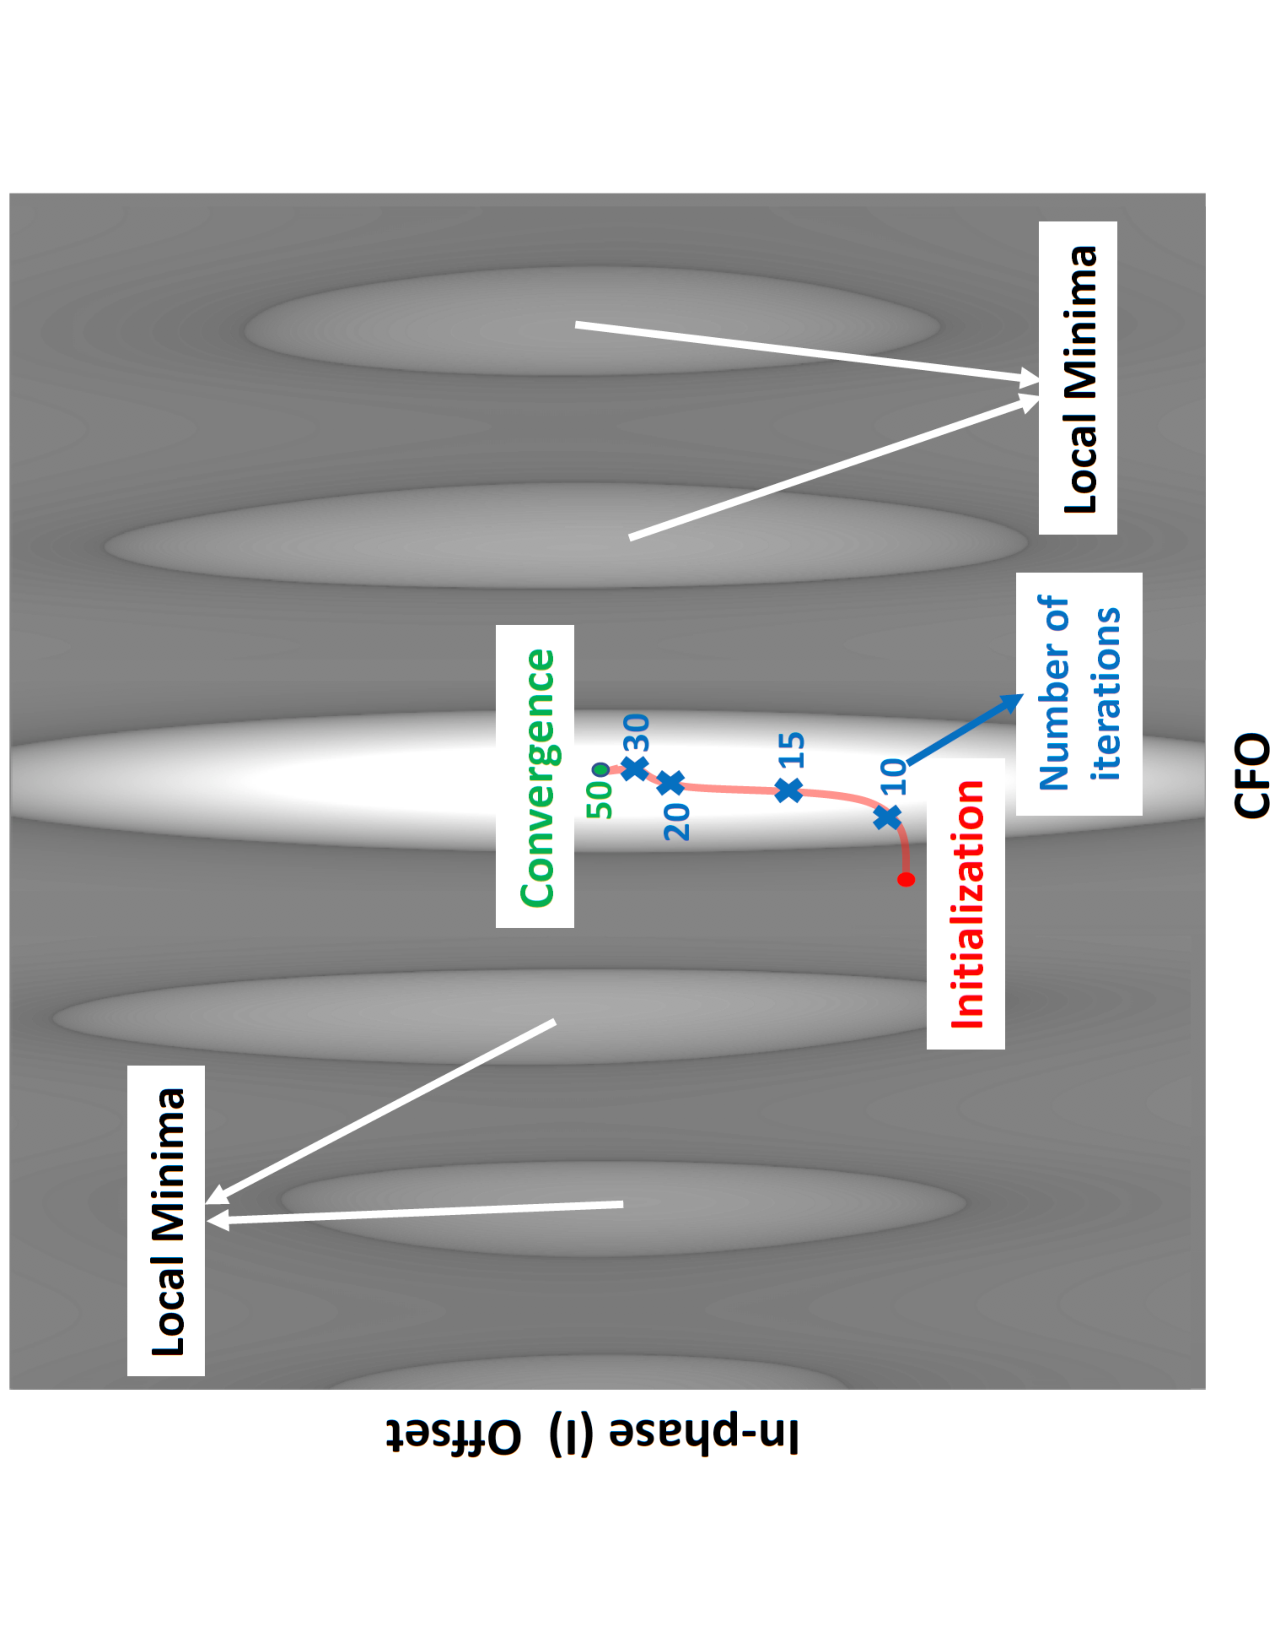
\includegraphics[angle = 270, width = \linewidth]{plots/heatmap.pdf} 
    \caption{Visualization of how the optimization based algorithm converges to the accurate hardware imperfection values such as CFO and IQ offset.}
    \label{fig:heatmap}
\end{figure}
Let $y = Real\{y\}+jImag\{y\}$ be the captured baseband signal (normalized by the average amplitude). In a GFSK modulated signal, ideally we have $Real\{y\} = cos(\omega(t)t)$ and $Imag\{x\} = sin(\omega(t)t)$ where $\omega(t)$ is the baseband frequency of the signal which is generated according to the GFSK modulation. However, the aforementioned hardware imperfections will slightly change the signal. We first decode the signal to obtain the sequence of bits and then, we make $\omega(t)$ according to GFSK modulation. Let $y'$ be the model of the imperfect signal. Considering the effects of CFO, IQ offset and IQ imbalance, we can write
\begin{gather*}
    y'(t) = A \times \big[(1-\frac{\epsilon}{2})cos(\omega(t)t-\frac{\phi}{2})+I+ \\
    j\big((1+\frac{\epsilon}{2})sin(\omega(t)t+\frac{\phi}{2})+Q\big)\big] \times e^{j(\phi_o+2\pi f_o t)}
\end{gather*}
where $f_o$, $\phi_o$, $A$, $\frac{1-\epsilon}{1+\epsilon}$, $\phi$, $I$ and $Q$ denote CFO, phase offset, normalized amplitude of the signal, IQ amplitude imbalance, IQ phase imbalance, I offset and Q offset, respectively. The goal is to choose the value of these variables in such a way that $||y'-y||^2$ is minimum and as a result, $y'$ is as close as possible to the captured signal $y$. Therefore, we must solve the following optimization problem:
\begin{gather*}
    min_{f_o,\phi_o,A,\epsilon,\phi,I,Q}{F=||y'-y||^2 =} \\ |Real\{y'\}-Real\{y\}|^2+|Imag\{y'\}-Imag\{y\}|^2
\end{gather*}
However, this problem is not convex and the objective function has several local minima as shown in Figure~\ref{fig:heatmap}. Consequently, any optimization technique may end up in a local optima. To avoid this, we initialize the variables properly to increase the chance of finding the global minimum significantly. Although theoretically it will not guarantee ending up in the global minimum for arbitrary optimum numbers of these variables, we found that in practice we will reach the optimum value with this initialization in practical conditions. 

To initialize CFO, start by taking the average of frequencies in the preamble. Then we compensate the initial CFO in the signal to get the signal $z = y e^{-2\pi f_o t}$. To estimate initial I/Q imperfections, we use the I/Q constellation of the GFSK signal. The I/Q constellation of an ideal GFSK signal is a circle centered at $(0,0)$ since the phase changes according to GFSK modulation but the amplitude is always constant. However, I/Q imperfection will change this constellation. Specifically, I/Q offset will shift the center of the circle as it is equivalent to adding a fixed complex term to the ideal signal, and IQ imbalance will change the shape from a circle to a tilted ellipse.
%
%These effects are shown in Figure~\ref{fig:iq_const}.
As a result, to get an initial estimation of IQ imperfections, we fit an ellipse to the 2-dimensional points $(Imag\{z\},Real\{z\})$ by minimizing the Least Square Error. The center of the ellipse will provide the initial IQ offset and initial IQ imbalance can be obtained from the ratio of minor and major diameter and rotation angle of the ellipse.\\

\if 0
\begin{figure}[t!]
    \centering
    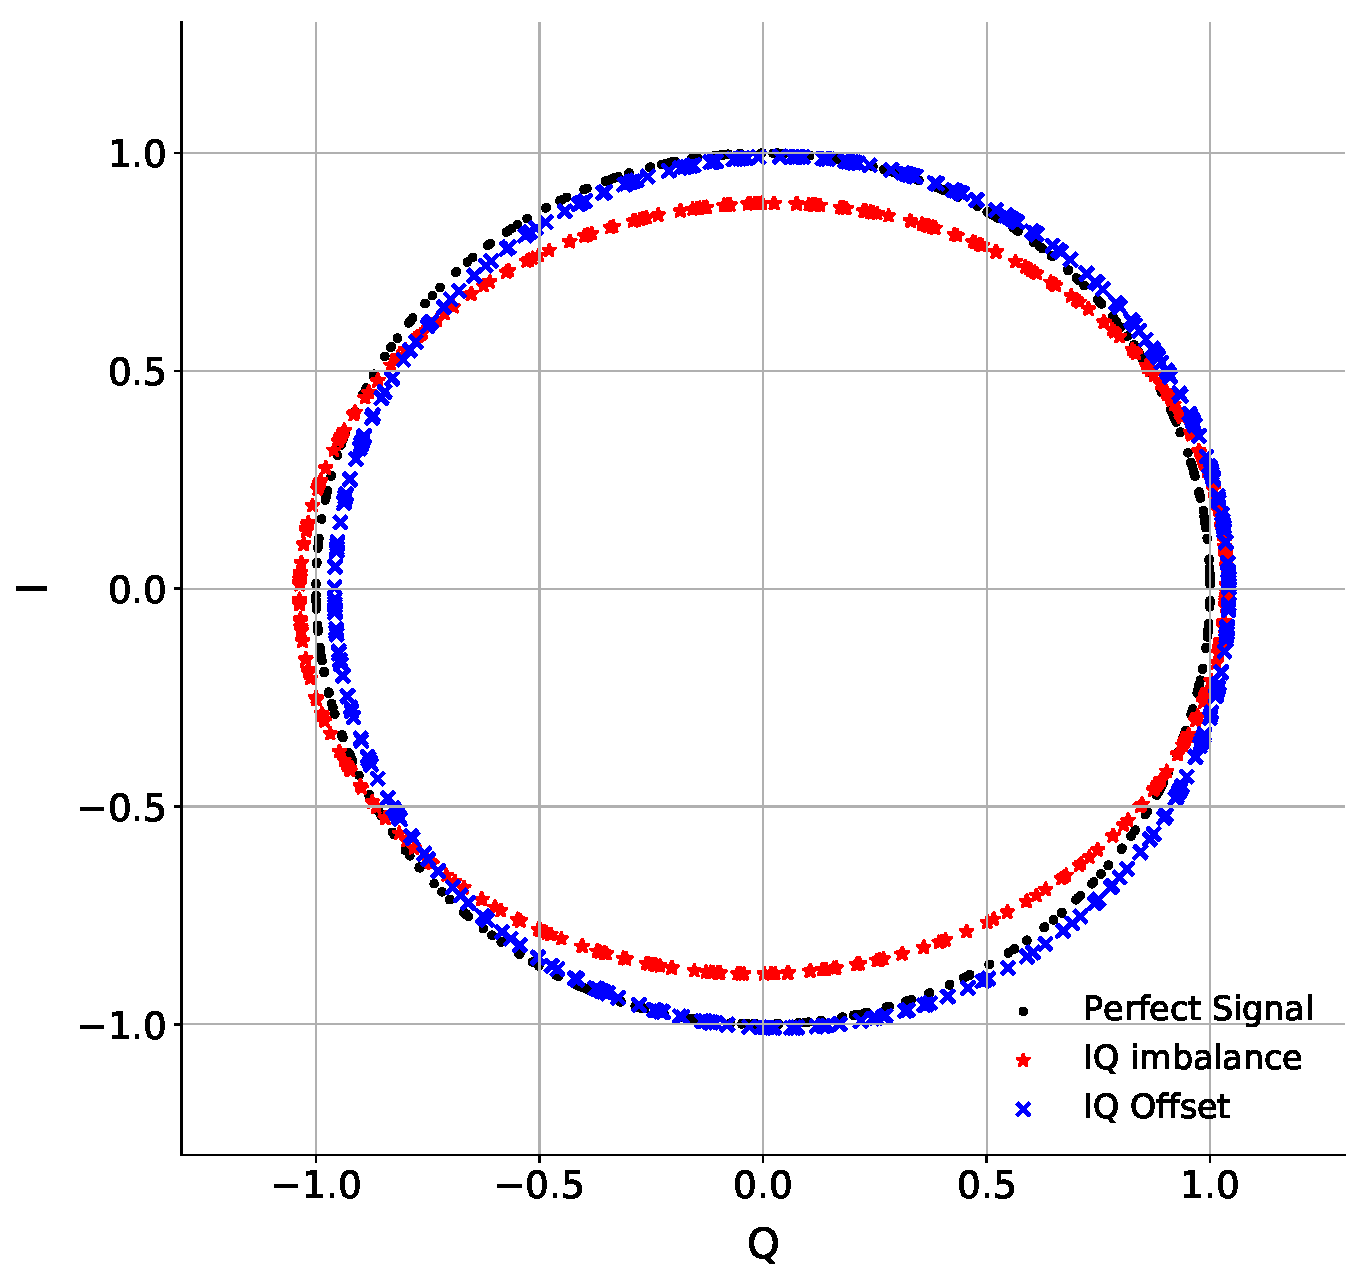
\includegraphics[width = \linewidth]{plots/IQ_const.pdf} 
    \caption{Effects of IQ imperfection on IQ constellation of a GFSK signal without noise and CFO}
    \label{fig:iq_const}
\end{figure}
%it will be long if I want to explain this ellipse thing
\fi

Although, these initial estimations provide an initialization close to optimum,
they are not accurate. 
%
As mentioned earlier, this initialization of CFO
is not accurate and robust enough as it only relies on an 8-microsecond
preamble. 
%
Also, mismatch in CFO compensation will cause a time-dependent phase
shift which distorts the I/Q constellation. 
%
Therefore, the initial IQ offset
and imbalance estimation will also have errors. 
%
Consequently, we employ
optimization techniques to jointly estimate hardware imperfection parameters
accurately and robustly. 
%
\noteby{NB-4}{
Finding these optimal values can be extremely computationally expensive. 
%
Indeed, the naive approach would be to brute force try all possible values for CFO, IQ offset and IQ imbalance to find the optimal values. 
%
Instead, we used gradient descent to solve the optimization problem, as it ensures that we move towards the optimal values after each step. 
%
Specifically, we use a widely-used fast form of gradient descent, Nesterov Accelerated Gradient Descent (NAG) to move from the initialization towards the optimum values
of $f_o,\phi_o,A,\epsilon,\phi,I,Q$ by minimizing $F$ in the mentioned
optimization problem. 
%
NAG adaptively adjusts the parameter update at each step, so that we move faster towards the optimal value at the start but slow down as we get close to the minima.}

\begin{comment}
Therefore, after this initialization, we use Nesterov
Accelerated Gradient Descent (NAG) to move from the initialization towards the optimum values
of $f_o,\phi_o,A,\epsilon,\phi,I,Q$ by minimizing $F$ in the mentioned
optimization problem. 
\end{comment}


Figure~\ref{fig:heatmap} demonstrates an instance of how we start from the initial estimations of CFO and IQ imperfections, move toward the optimal values of CFO and IQ imperfections using gradient descent (the red line), and converge to the accurate estimations of CFO and IQ imperfections in a few iterations.


% TOO LONG ====================
%However, as mentioned earlier, this optimization problem is convex and we may converge to the local optima. Therefore, if after convergence, the average of $F$ was not less than a certain threshold which is determined according to SNR, we add certain steps to the first initialization and repeat the aforementioned gradients descent process. We keep searching for the optimum with new initializations until either the average of $F$ falls below the threshold or our initialization falls out of the bound of the typical values for these imperfections (in which case we give up on the packet. This typically happens when the SNR is less than 5 dB or there is a collision). The first initialization will increase the speed of convergence as usually it will be close to the optimum and re-initialization will ensure ending up in a point which is either the global optimum or very close to global optimum (in the sense that the objective function is less than the desired threshold and hence, is within a small margin of global optimum). The proposed algorithm fulfills the two key properties that we explained at the beginning of this subsection. First, the NAG based joint estimation of CFO and IQ imperfections ensures precise estimation with fine granularity as it keeps moving towards the optimum with adaptive steps and removes the mutual effect of mismatch in estimating these imperfection parameters. Second, the objective function of optimization is chosen as the summation of all PHY samples across the packet, which diminishes the impact of AWGN and provide more robust information and granularity. The final result is achievement of a highly precise CFO and IQ estimates for a device, that are robust to environmental noise, and can therefore be used by an attacker as a unique fingerprint for generic consumer devices.
% Shorter ==========
However, as mentioned earlier, this optimization problem is not convex and we may converge to the local optima. Therefore, if after convergence, the average of F was not less than a certain threshold which is determined according to SNR, we add certain steps to the first initialization and repeat the aforementioned gradients descent process. The proposed optimization based estimation ensures accurate estimation with fine granularity as it keeps moving towards the optimum with adaptive steps and removes the mutual effect of mismatch in estimating these imperfection parameters. Moreover, the objective function of optimization is chosen as the summation of all PHY samples across the packet, which diminishes the impact of AWGN and provide more robust information and granularity.

% This is restated, so cutting other eval is there now
\if 0
We use this methods to extract CFO, IQ offset and IQ imbalance for 20 ESP32 chipsets of the same make and model. Figure~\ref{fig:esp} represents CFO and IQ offset magnitude for 10 packets for each of these 20 chipsets. The low variance of CFO for each device, shows these methods is very accurate in measuring hardware imperfections (e.g. the CFO standard deviation average for 20 devices is 200 Hz in our algorithm which is significantly less than the existing methods described earlier). Obviously, low within-class variance will significantly improve the identification accuracy and these 20 devices can be clearly distinguished only by their CFO and IQ offset. 
\fi

\vspace{0.5em}
\noindent\textbf{Summary:} For the first time we showed that it is feasible to estimate CFO and IQ imperfections of WiFi/BLE combo chipsets accurately based on the simple BLE signal itself; in other words, without needing the rich signal features that are present in WiFi.


\subsubsection{Profiling and identifying the device}
\label{sec:methodology2}

The first step in deploying our RF fingerprinting attack is to capture the BLE signal. We use an SDR to capture raw I and Q samples of BLE. Next, we use the captured signal to fingerprint the device. The entire processing flow can be divided into two stages, Fingerprinting Stage and Identification Stage. In the former stage, the device is isolated and we capture a number of packets from the target device to build a profile for the device (training packets). The latter stage, employs this profile to identify the device when the MAC addresses is changed.

\vspace{0.5em}
\noindent\textbf{Fingerprinting Stage:} For each packet from a device $D$, CFO and IQ imperfections can be extracted with a high resolution using algorithm described in~\ref{sec:methodology1}. Let $x_1,...,x_N$ be the CFO and IQ imperfection feature vectors for $N$ training packets we have received from device $D$. We calculate the mean $\mu_D$ and covariance matrix $\Sigma_D$ of $X = [x_1 \quad ... \quad x_N]$. $\mu_D$ and $\Sigma_D$ together with a threshold that will be defined later is considered the profile of device $D$.

\noindent\textbf{Identification Stage:} In identification stage, we want to decide whether a packet $x_t$ with a new MAC address belongs to device $D$, indicating that the target device is present. To do so, we compute the Mahalanobis distance to the profile of device $D$

\begin{gather*}
    distance(x_t,\mu_D,\Sigma_D) = \sqrt{(x_t-\mu_D)^T\Sigma_D^{-1}(x_t-\mu_D)}
\end{gather*}


This distance is a way to measure how close the features of the new packet are to the profile of device $D$. In addition to $\mu_D$ and $\Sigma_D$, we define a threshold $thresh$ as the profile of the device. Whenever $distance(x_t,\mu_D,\Sigma_D)<thresh$, packet $x_t$ belongs to the target device $D$ and device $D$ is identified. Otherwise, packet $x_t$ belongs to some other device in the world that we are not looking for. This threshold is chosen using the validation set. One could choose a threshold that guarantees a certain level of FNR according to the validation set. Another way is to pick a threshold that balances both FPR and FNR. To obtain that goal, we pick the threshold that minimizes $FPR^2+FNR^2$ so that neither FNR nor FPR gets much larger than the other. In this paper, we use these two methods for selecting the threshold depending on the goal of analysis in different experiments.


Moreover, since the MAC address is fixed for a period of time, we receive a number of packets with the same MAC address which we know belong to the same device. As a result, we can make a decision about the identity of the MAC address instead of the individual packets. One way that we found most effective, was to first average the feature vector $x$ for all packets with the same MAC address and then compute the Mahalanobis distance. This would further reduce the tolerance due to estimation error and inherent tolerance of features.

\if 0 % extra {{{
\paragraph{Fingerprinting Stage} For each packet from a device $D$, CFO anf IQ imperfections (IQ offset and IQ imbalance) can be extracted with a high resolution using algorithm described in~\ref{sec:methodology1}. Let $x_1,...,x_N$ be the CFO and IQ imperfection feature vectors for $N$ training packets we have received from device $D$. We calculate the mean $\mu_D$ and covariance matrix $\Sigma_D$ of $X = [x_1 \quad ... \quad x_N]$. $\mu_D$ and $\Sigma_D$ together with a threshold that will be defined later is considered as the profile of device $D$.



%Note that IQ offset and imbalance are only useful for combo transmitters and will be ignored by classifier while classifying BLE-only transmitters.
\paragraph{Identification Stage} In identification stage, we want to decide whether a packet $x_t$ with a new MAC address belongs to device $D$, indicating that the target device is present. To do so, we compute the Mahalanobis distance to the profile of device $D$

\begin{gather*}
    distance(x_t,\mu_D,\Sigma_D) = \sqrt{(x_t-\mu_D)^T\Sigma_D^{-1}(x_t-\mu_D)}
\end{gather*}
\begin{gather*}
    distance(x_t,\mu_D,\Sigma_D) = \sqrt{(x_t-\mu_D)^T\Sigma_D^{-1}(x_t-\mu_D)}
\end{gather*}
%This is assuming that the estimated CFO and IQ imperfections have a Gaussian distribution which is a fair assumption considering that the tolerance in CFO and IQ imperfection estimation of a device for different packets is mainly caused by variations in SNR (which affects estimation error) and tolerance of the underlying hardwar.
This distance is one way to measure how close the features of the new packet are to the profile of device $D$. In addition to $\mu_D$ and $\Sigma_D$, we define a threshold $thresh$ as the profile of the device. Whenever $distance(x_t,\mu_D,\Sigma_D)<thresh$, packet $x_t$ belongs to the target device $D$ and device $D$ is identified. Otherwise, packet $x_t$ belongs to some other device in the world that we are not looking for. This threshold is chosen using the validation set.
Moreover, since the MAC address is fixed for a period of time, we receive a number of packets with the same MAC address which we know belong to the same device. As a result, we can make a decision about the identity of the MAC address instead of the individual packets. One way that we found most effective, was to first average the feature vector $x$ for all packets with the same MAC address and then compute the Mahalanobis distance. This would further reduce the tolerance due to estimation error and inherent tolerance of features.


\fi
%}}}

\subsubsection{Comparing CFO accuracy} %{{{
\begin{figure}[t!]
    \centering
    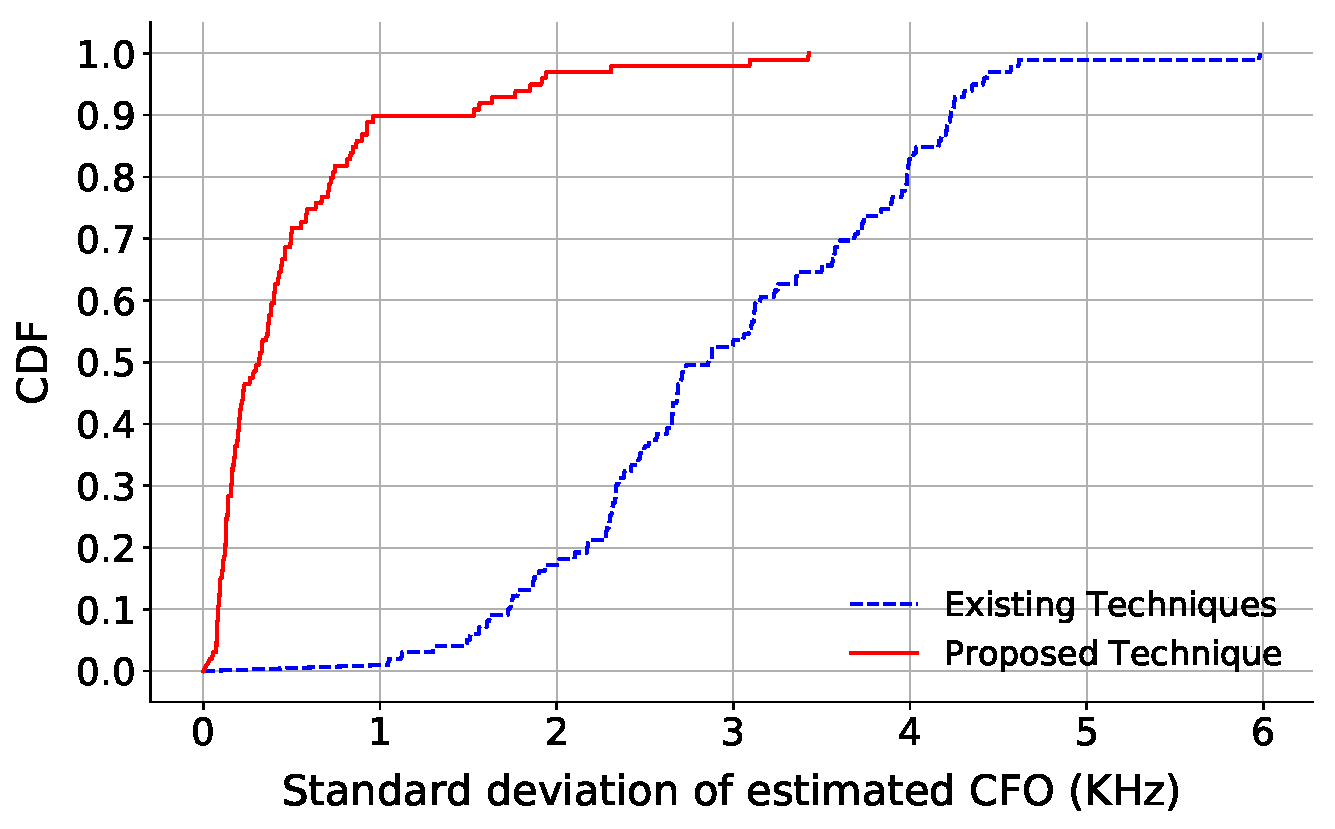
\includegraphics[width = \linewidth]{plots/CFO_comparison_ESP.pdf} 
    \caption{Comparing the CFO estimation of existing coarse-grained techniques with our proposed technique.}
    \label{fig:cfo_comp}
\end{figure}


%
To evaluate the accuracy of our new fine-grained fingerprinting algorithm compared to coarse-grained BLE
CFO estimation, 
we compute CFO for 100 packets from 100 of BLE transmitters observed in the field.% For each device, we
%consider the CFO estimation technique which yielded the lowest standard deviation (std).
%
Figure~\ref{fig:cfo_comp} shows the CDF of the standard deviation of CFO for both techniques.
%
We see that 
our fine-grained CFO estimation significantly reduced the standard deviation of CFO estimation for all devices. This reduces the within-class variance and
makes these devices have significantly more unique fingerprints.
%Moreover, as inaccurate estimation and compensation of
%CFO affects the estimation of IQ imperfections since the residual CFO will
%cause IQ samples to rotate by time.
% In fact, no prior work has
%demonstrated that it is possible to obtain accurate and identifiable estimates
%of imperfections for BLE transmitters.
%
%Consequently, we must develop a new
%algorithm to enable find-grained and robust estimation of CFO and IQ
%imperfections to enable our device identification attack.

%The resulting standard deviation of the measured CFO was 1.5 KHz (we averaged the CFO standard deviation across 20 different devices). This standard deviation is huge for performing the task of RF fingeprinting and will end up in low accuracy of identifying devices based on RF fingerprints. 
%}}}
\subsubsection{Why not simply neural nets?}
\noteby{NB-3}{
Indeed, early in the work, we tried neural networks as an identification technique. However, they made it difficult to carry out the attack. Also, they limited our ability to perform a detailed evaluation of the strengths and limitations of each of the individual types of hardware imperfections that we can use for device identification. Some of the issues we will describe are as follows:
}

\noteby{NB-3}{
(1) Neural network training can overfit to a specific bit pattern in a packet. This is a problem because BLE advertisements do not have a stable bit pattern. For example, BLE packets from a single device change every 15 minutes when the device’s MAC address re-randomizes. Our technique is not dependent on the data in the packets because we classify devices based only on their hardware imperfections, not their packet data.
}

\noteby{NB-3}{
(2) Neural networks make it difficult to determine the significance and distinguishability of each type of hardware imperfection (e.g. CFO, IQ offset) in identification accuracy. Our method directly estimates these hardware imperfection features themselves, making it possible for us to individually study them. This allowed us to study the separability of devices by each aspect of imperfections (e.g., I/Q offset and CFO), the relative importance of each imperfection for identification, how the imperfections are affected by temperature, and how accurately they can be captured by a low-cost SDR.
}

\noteby{NB-3}{
(3) Neural nets are less practical for a tracking attack than the method we proposed. Our preliminary experiments with neural nets indicated that they require significantly more training data than the conventional classification we describe.
}
